\section{Thursday, April 4th}
\subsection{Logistics}
\begin{itemize}
    \item Review Reviews
    \item Discussion Posted
    \item Project Update due next Thursday
    \item Quiz 6 Today
\end{itemize}

\subsection{Information and Thermodynamics}
Consider the second law of thermodynamics, which states "entropy always increases". We want to formalize this. What exactly are we computing the entropy of? We need to take into account the random variable, distribution and the overall state of the system. Does it increase always or under certain assumptions?

The big question is if thermodynamic entropy can be related to the notion of entropy that we have developed so far. 

\subsection{Naive Approach}
Let's try a Markov Chain approach! We'll start simple with just two states and work in discrete time. Imagine a Markov chain with two states $\boxed1$ and $\boxed2$. Let's assume transitions $p_{11}, p_{12}, p_{21}$ and $p_{22}$ are all nonnegative. Assume WLOG that $p_{21}>>p_{11}>0$ and $p_{22} >> p_{12}>0$. 

Note that the steady state behaviour of this system basically sets $p^*_{22}=1$ and $p^*_{11} = 0$ in the limit of these two assumptions. We would like to say that the entropy of some quantity is increasing in time. 

Consider the entropy of $X(t)$. Clearly $H[X(t)] = 0$ in the limit since all of the probability mass is concentrated at $\boxed2$. However, imagine if we started the process with an initial uniform distribution? 

Then we have just decreased the entropy! We have designed a process that starts with maximal entropy and reduces all the way to $0$ entropy. 

\subsection{Thermodynamics}

What is Thermo? We are not talking about your average thermoflask here. It is a statistical theory for dynamics of macroscopic observable. It studies quantities of heat, energy, temperature and pressure. Microstate refers to the detailed model. However, this is completely intractable. You want to think about this as your average Tall drink in Starbucks. 

Mesoscopic states refers to "mid-sized" process. Think of this as your average Grande drink from Starbucks. 

Macroscopic state refers to the state where you average out the randomness and go to the limit of having infinite particles. Think of this as your average Venti drink from Starbucks. 

\subsection{Picking a System for the Mesoscopic State}
\subsubsection{Microscopic vs Mesoscopic vs Macroscopic}
\begin{figure}[H]
    \centering
    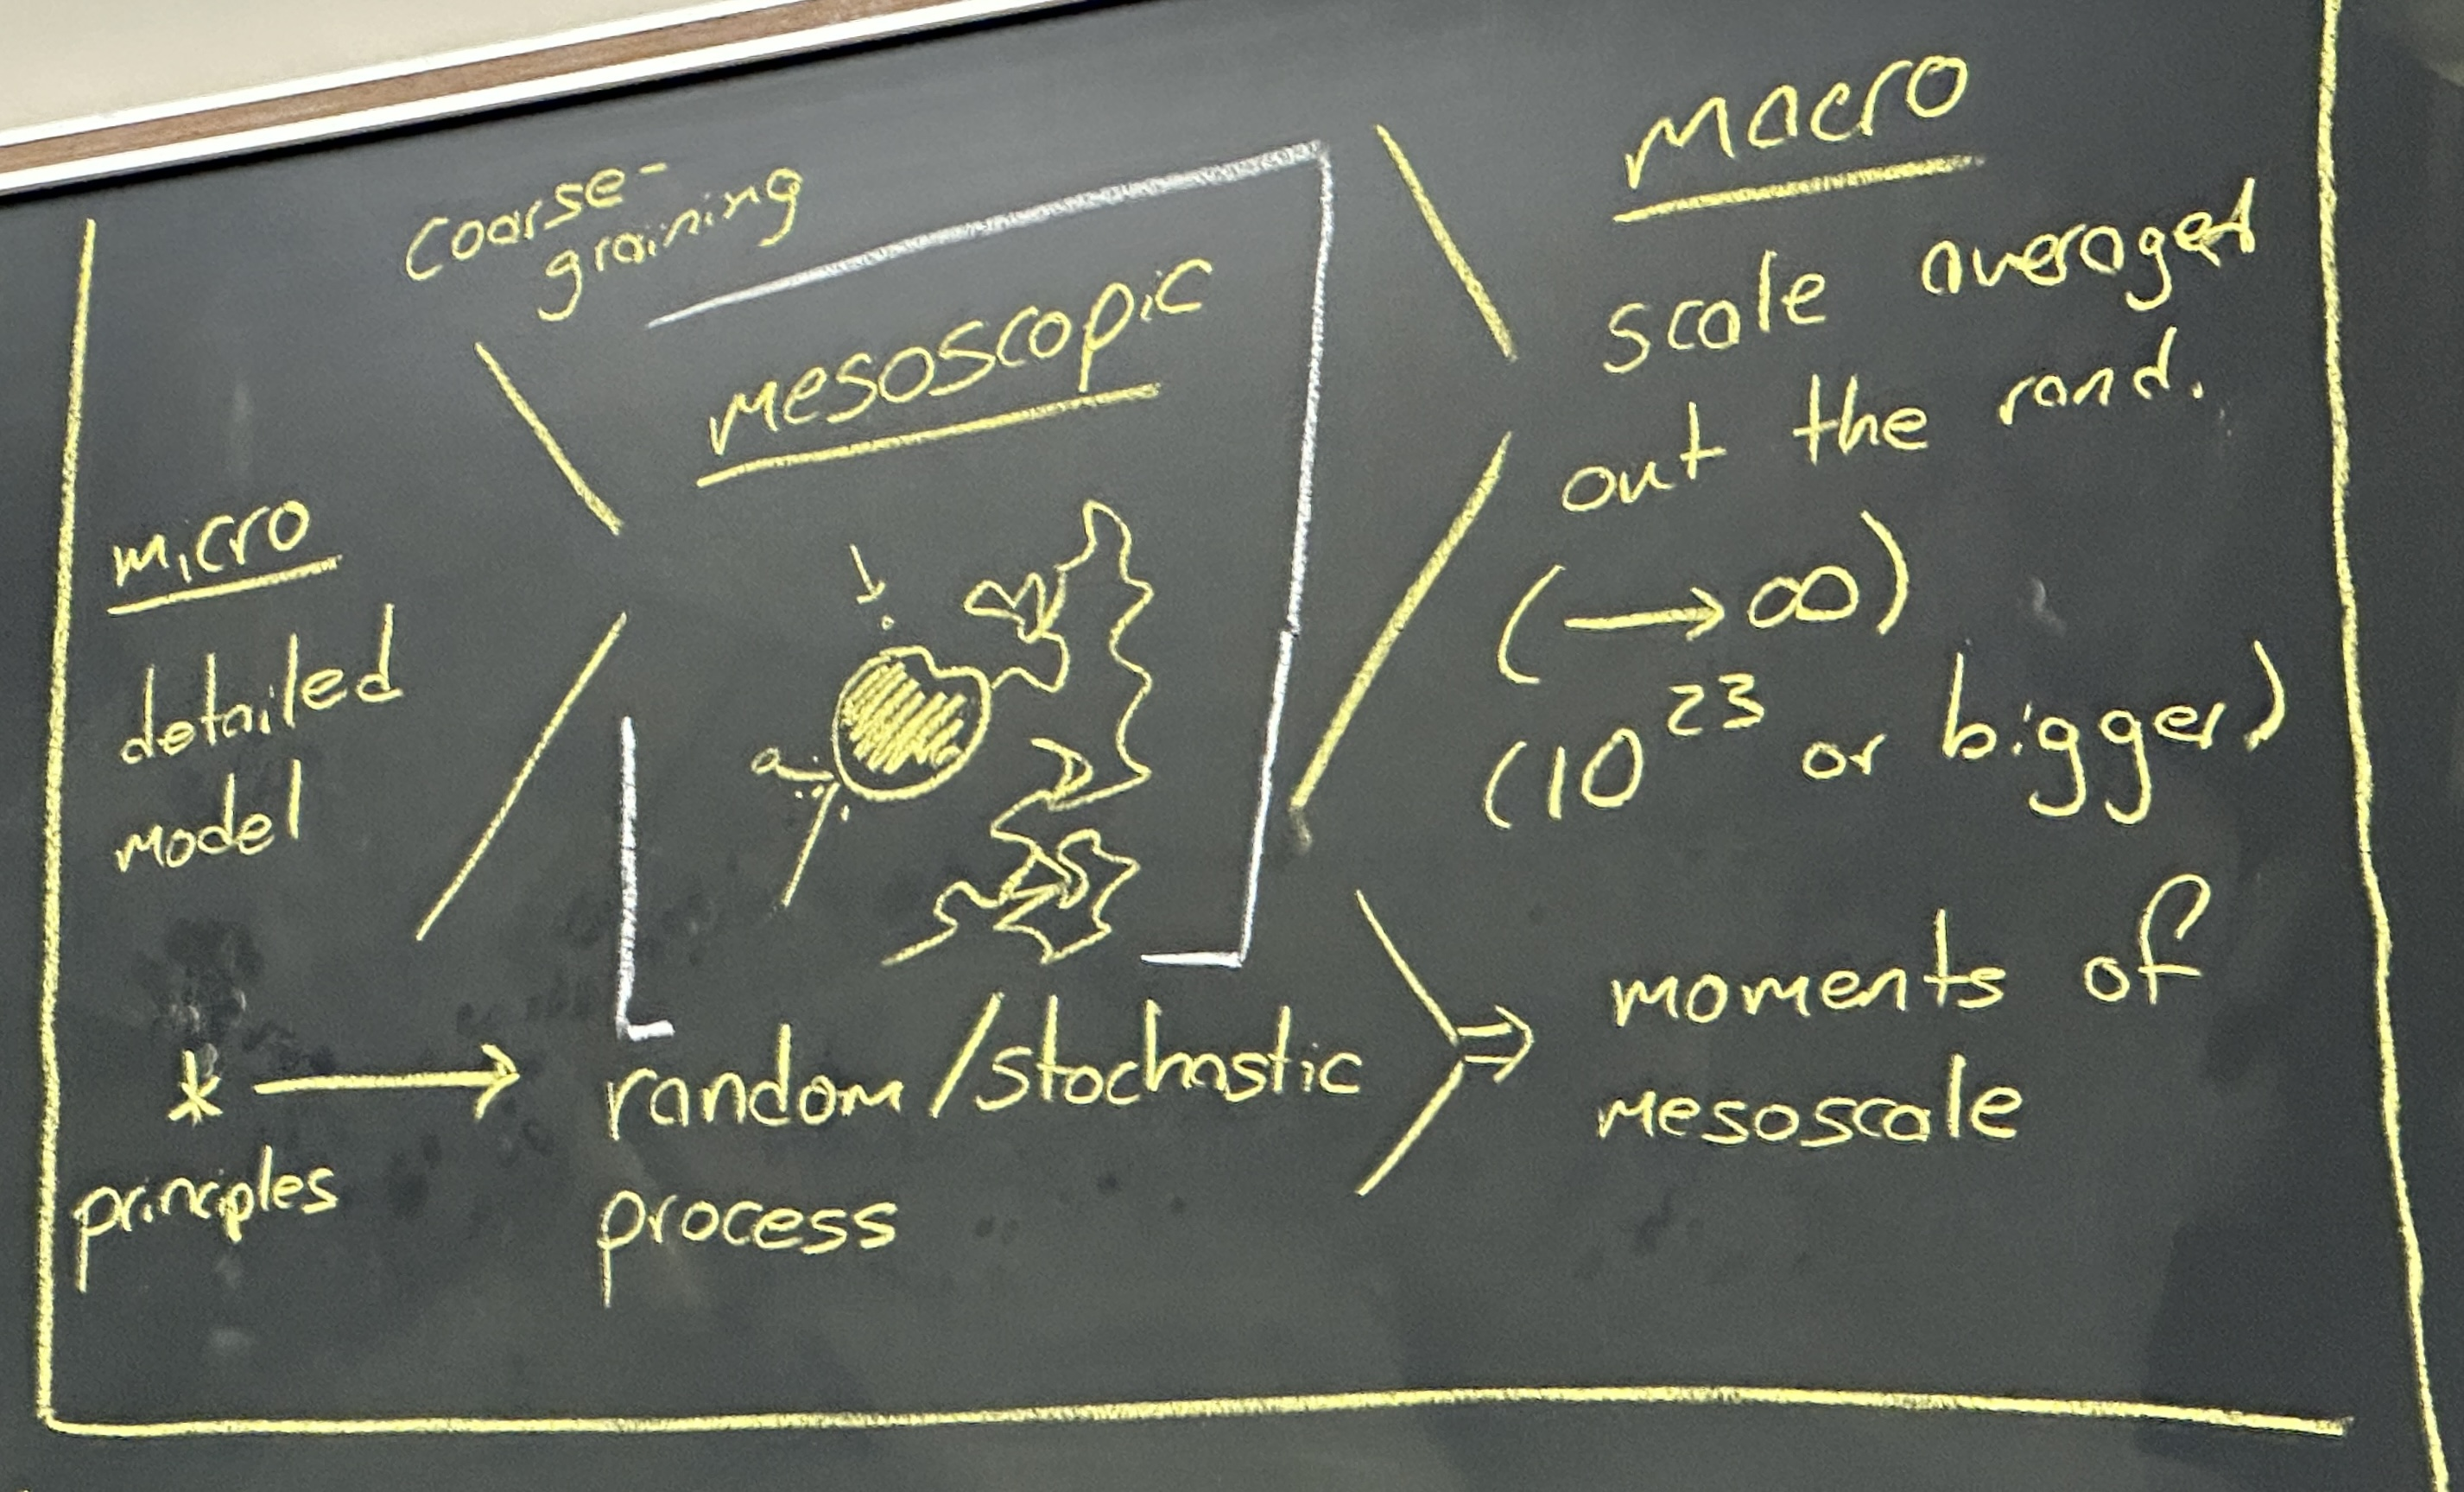
\includegraphics[scale=0.152]{lectures/wk11/img/meso.jpeg}
    % \caption{Caption}
    \label{fig:micro-meso-macro}
\end{figure}



\subsection{Continuous Time Markov Chains}
$X(t)$ is a jump process. 

\begin{itemize}
    \item Waiting times are exponentially distributed : $T_j \sim \Exp(\sum_{k\neq j} r_{kj})=\Exp(R_j)$.
    $R_j = \sum_{k \neq j} r_{kj}$

    \item Prob jump from $j \rightarrow k$ is $ \frac{r_{kj}}{R_j}$

    \item Then: transition rate matrix: $R = 
    \begin{cases}
        r_{ij} &= \mathrm{rate } j \rightarrow i \\
        r_{ii} &= -R_i = - \sum_{k \neq i} r_{k_i}
    \end{cases}
    $

    \item Master Equation: Let $p(t) = \mathrm{dist } X(t), X(0) \sim p(0)$ then: $ \dv{}{t}p(t) = Rp(t)$ so: $p(t) = e^{Rt} p(0)$

    \item Steady-State: $P_s$ s.t. if $X(0) \sim p_s, X(t) \sim p_s$ solution to $: Rp_s = 0$

    \item Flux-Balance: flux $j \rightarrow i = r_{ij} p(x_j, t)$

    \item Complex-Balance: $ \sum_{j \neq i} r_{ij} P_s(j) = R_i P_s(i) $

    \item Discretization: $p_n = \mathrm{dist } X_n = X(t_n)$
    if $t_n = n \Delta t$ then $X_n$ is a discrete time MC with transition prob matrix $P(\Delta t) = e^{R \Delta t}$
\end{itemize}

\begin{shaded}
What are the barebones addtl. assumptions to introduce to our stoch proc at the microscopic scale to satisfy sensible mesoscopic scale dynamics?
\end{shaded}

\subsection{Conservation Laws}
\begin{itemize}
    \item total mass is conserved
    \item momento (momentum) is conserved
    \item energy is conserved -- it cannot be created nor destroyed -- but \textit{why}? 
\end{itemize}

\subsection{Required Symmetries}
\begin{enumerate}
    \item If I knew every detail of the current state, then I would know the rule for how it changes $\implies$ dynamics only depend on the current-state.
    \item The process evolves in cts.-time.
    \item If we knew or could track all relevant d.o.f. then the dynamics would be \textit{time autonomous}.
    \item Time-Reversibility: Your dynamical rules (updates to your system) should be symmetric if you reverse time. This is what implies the conservation of energy.
\end{enumerate}

\subsection{Noether's Theorem}
Every continuous symmetry of the action of a physical system with conservative forces has a corresponding conservation law.

Translational symmetry $\mapsto$ Conservation of momentum.

Rotational symmetry $\mapsto$ Conservation of angular momentum.

Time-Translational symmetry $\mapsto$ Conservation of total energy.

% If your mesoscopic process is markov then your microscopic process will be Markov.
% 
If your microscopic process is markov then your mesoscopic process will be Markov.
